%@descr: wzór sprawozdania, raportu lub pracy - nadaje się do przeróbek
%@author: Maciej Komosiński

\documentclass{article} 
\usepackage{polski} 
\usepackage[utf8]{inputenc} 
\usepackage[OT4]{fontenc} 
\usepackage{graphicx,color} %include pdf's (and png's for raster graphics... avoid raster graphics!) 
\usepackage{url}
\usepackage{float}
\usepackage[pdftex,hyperfootnotes=false,pdfborder={0 0 0}]{hyperref} %za wszystkimi pakietami; pdfborder nie wszedzie tak samo zaimplementowane bo specyfikacja nieprecyzyjna; pod miktex'em po prostu nie widac wtedy ramek


% Zmiana rozmiarów strony tekstu
\addtolength{\voffset}{-1cm}
\addtolength{\hoffset}{-1cm}
\addtolength{\textwidth}{2cm}
\addtolength{\textheight}{2cm}

%bardziej zyciowe parametry sterujace rozmieszczeniem rysunkow
\renewcommand{\topfraction}{.85}
\renewcommand{\bottomfraction}{.7}
\renewcommand{\textfraction}{.15}
\renewcommand{\floatpagefraction}{.66}
\renewcommand{\dbltopfraction}{.66}
\renewcommand{\dblfloatpagefraction}{.66}
\setcounter{topnumber}{9}
\setcounter{bottomnumber}{9}
\setcounter{totalnumber}{20}
\setcounter{dbltopnumber}{9}

% własny bullet list z malymi odstepami
\newenvironment{tightlist}{
\begin{itemize}
  \setlength{\itemsep}{1pt}
  \setlength{\parskip}{0pt}
  \setlength{\parsep}{0pt}}
{\end{itemize}}

%obrazkow szukamy w nastepujacym katalogu:
\graphicspath{{pics/}}



%\title{Sprawozdanie z laboratorium:\\Metaheurystyki i Obliczenia Inspirowane Biologicznie}
%\author{}
%\date{}


\begin{document}

\thispagestyle{empty} %bez numeru strony

\begin{center}
{\large{Sprawozdanie z laboratorium:\\
Metaheurystyki i obliczenia inspirowane biologicznie}}

\vspace{3ex}

Część I: Algorytmy optymalizacji lokalnej, problem ATSP
%Część II: Algorytmy optymalizacji lokalnej i globalnej, problem QAP
%Część III: Eksperyment: ... (prezentację można zrobić w LaTeX - służy do tego klasa "beamer")

\vspace{3ex}
{\footnotesize\today}

\end{center}


\vspace{10ex}

Prowadzący: dr hab.~inż. Maciej Komosiński

\vspace{5ex}

Autorzy:
\begin{tabular}{lllr}
    \textbf{Marcin Mrugas} & inf122580 & marcin.mrugas@student.put.poznan.pl \\
    \textbf{Piotr Kicki} & inf122401 & piotr.kicki@student.put.poznan.pl \\
\end{tabular}

\vspace{5ex}

Zajęcia środowe, 16:50.

\vspace{35ex}

\noindent Oświadczam/y, że niniejsze sprawozdanie zostało przygotowane wyłącznie przez powyższych autora/ów,
a wszystkie elementy pochodzące z innych źródeł zostały odpowiednio zaznaczone i~są cytowane w bibliografii.  

\newpage


\section*{Udział autorów}
\begin{tightlist}
    \item MM zaimplementował szkielet aplikacji, oraz przeszukiwanie losowe, przeprowadził eksperyment z podobieństwem, opisał eksperymenty
    \item PK zaimplementował przeszukiwanie lokalne, przeprowadziła eksperyment najlepszych i średnich wyników algorytmów, opisała...,
\end{tightlist}


\section{Wstęp}

Naszym zadaniem było zaimplementowanie i przestudiowanie asymetrycznego problemu komiwojażera. Problem ten polega na znalezieniu najkrótszego cyklu Hamiltona w grafie asymetrycznym. Można go interpretować jako logistyczny problem dotyczący znalezienia takiej trasy dla dostawcy, aby ten odwiedził wszystkich odbiorców w jak najkrótszym czasie. Problem należy do klasy problemów NP-zupełnych. Złożoność tego problemu, w najgorszym przypadku, sprowadza się do przeglądnięcia wszystkich cyklów Hamiltona których dla grafu o zupełnego o $n$ wierzchołkach jest $n!$. Dlatego problem ten optymalizuje się algorytmami które w przestrzeni rozwiązań starają się rozważać mniejszą część rozwiązań i uzyskują rozwiązania często gorsze od optymalnego ale osiągają ten wynik w znacznie krótszym czasie.

\begin{figure}[H]
\begin{center}
    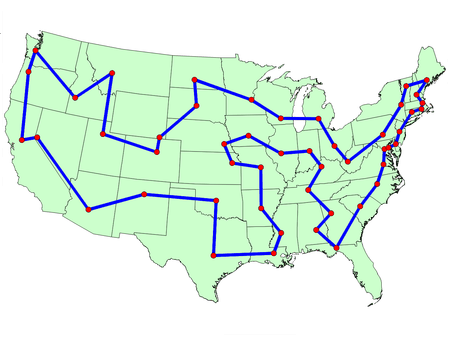
\includegraphics[width=0.7\textwidth]{map002g.png}
\end{center}
\caption{Przykładowe rozwiązanie problemu komiwojażera ze stolicami stanów Stanów Zjednoczonych.}
\label{fig:schemat}
\end{figure}

\section{Instancje}

Eksperymenty zostały przeprowadzone na wszystkich dostępnych instancjach.

\section{Opis sąsiedztwa}

Operatorem sąsiedztwa w naszej implementacji jest 2-OPT. Nowy sąsiad jest tworzony poprzez zamianę miejscami dwóch wierzchołków rozwiązania. 

\begin{figure} 
\begin{center}
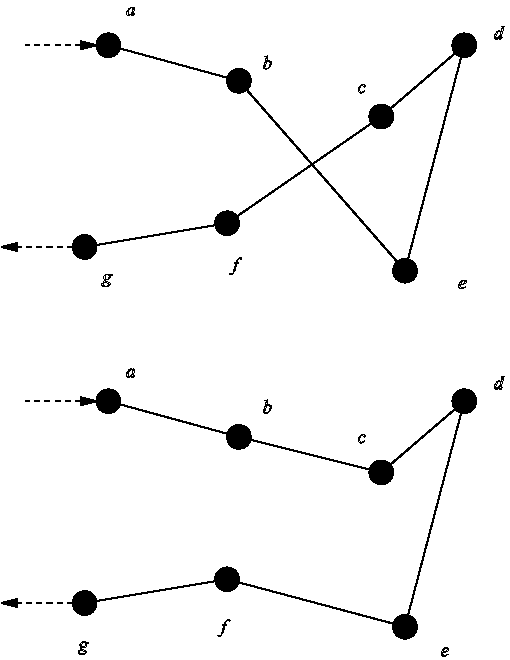
\includegraphics[width=0.4\textwidth]{twooptwiki.pdf}
\end{center}
\caption{Przykład sąsiedztwa.}
\label{fig:schemat2}
\end{figure}


\section{Porównanie działania algorytmów}


\subsection{Jakość}
Za miarę jakości obraliśmy wartość równania:
$$ \frac{\eta}{\eta_{min}}-1 $$
gdzie:\\
$\eta_{min}$ -- długość optimum globalnego \\
$\eta$ -- długość rozważanego rozwiązania

Co można interpretować jako wartość o jaką długość rozwiązania $\eta$ jest procentowo dłuższa od rozwiązania optymalnego $\eta_{min}$

\begin{figure}[H]
\begin{center}
    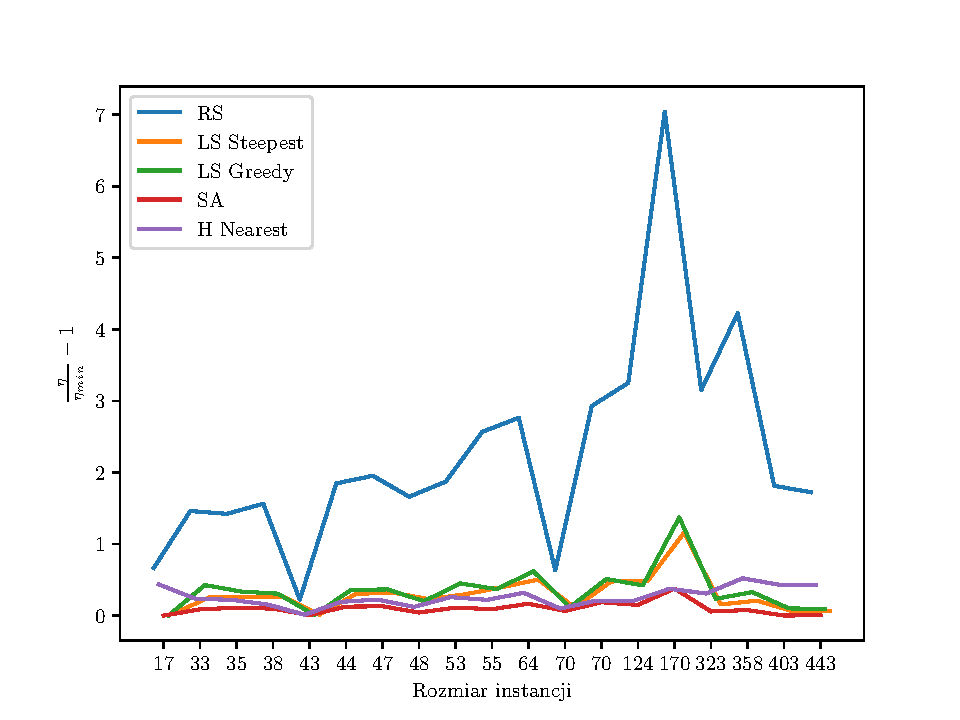
\includegraphics[width=1\textwidth]{plot_min.pdf}
\end{center}
\caption{Najlepsze uzyskane wyniki.}
\label{fig:plot_min}
\end{figure}

Na rys. \ref{fig:plot_min} przedstawiono wykres zawierający najlepsze wyniki z 10 uruchomień algorytmów. Na wykresie można zauważyć że najgorsze wyniki daje algorytm Random Search, który uzyskuje średnio jakość 1 - 2 czyli dwukrotnie gorsze rozwiązanie od optymalnego oraz 8 razy gorsze w najgorszym przypadku. Pozostałe algorytmy dawały bardzo podobne do siebie rezultaty czyli o 30\% gorsze od rozwiązania optymalnego. Dodatkowo dla największych instancji algorytm heurystyczny dawał gorsze wyniki niż algorytm lokalny.

\begin{figure}[H]
\begin{center}
    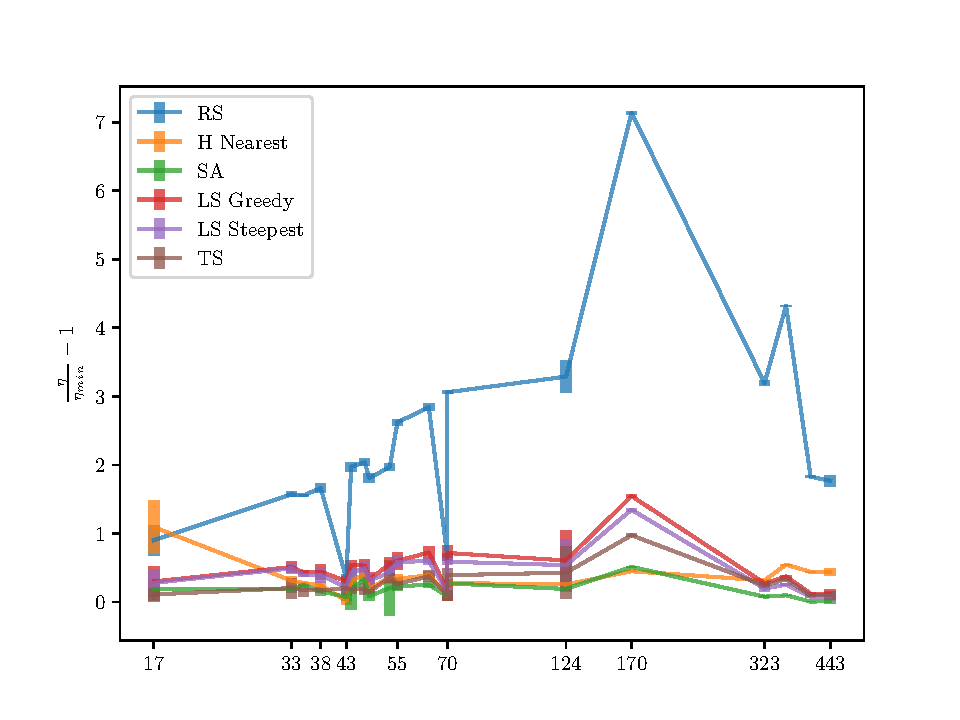
\includegraphics[width=1\textwidth]{plot_mean.pdf}
\end{center}
\caption{Średnie wyniki algorytmów}
\label{fig:plot_avg}
\end{figure}


Na rys. \ref{fig:plot_avg} zostały przedstawione średnie wyniki algorytmów. Dla czytelności rozmiary instancji są pokazane w skali logarytmicznej. Z wykresu widać że algorytm losowy znowu dawał najgorsze wyniki, algorytmy lokalne działały bardzo podobnie na korzyść algorytmu steepest. Można także zauważyć że instancja o rozmiarze 124 była dość trudna bo algorytmy otrzymywały rozwiązania o bardzo różnorodnej długości.

\subsection{Czas działania}

\begin{figure}[H]
\begin{center}
    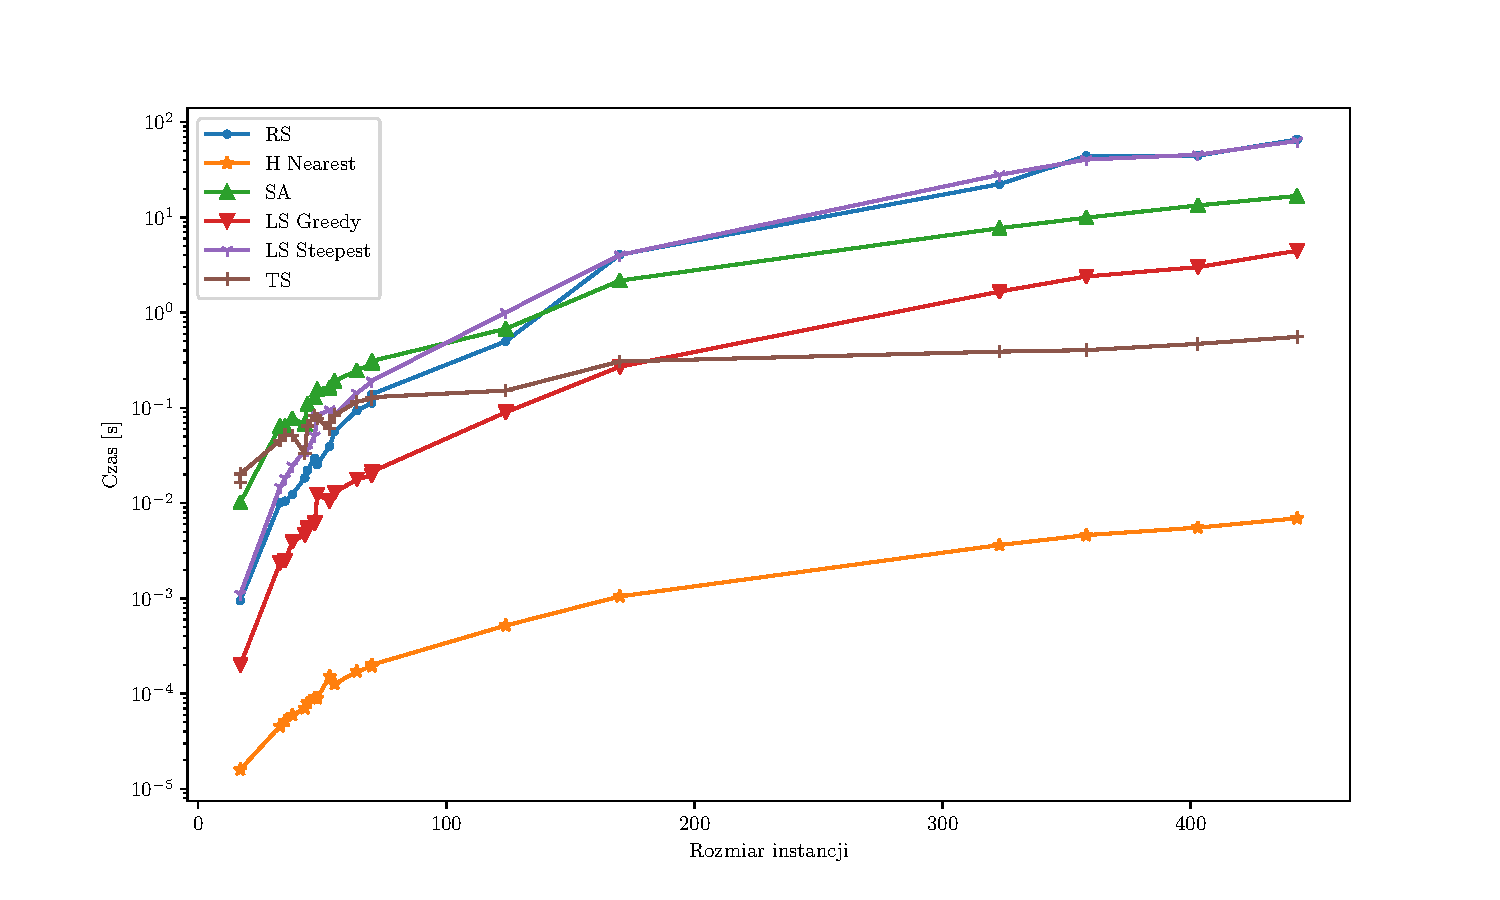
\includegraphics[width=1\textwidth]{plot_mean_time.pdf}
\end{center}
\caption{Czas działania algorytmów}
\label{fig:plot_time}
\end{figure}

Rys. \ref{fig:plot_time} Przedstawia czas działania algorytmów. Naszybciej działał algorytm heurystyczny, następnie Greedy i na końcu Steepest. Czas działania algorytmu losowego był dobrany tak aby działał porównywalnie długo jak algorytm lokalny. Widać także że czas działania algorytmów rośnie wykładniczo, gdyż wykres jest wyskalowany logarytmicznie.


\subsection{Efektywność}


\begin{figure}[H]
\begin{center}
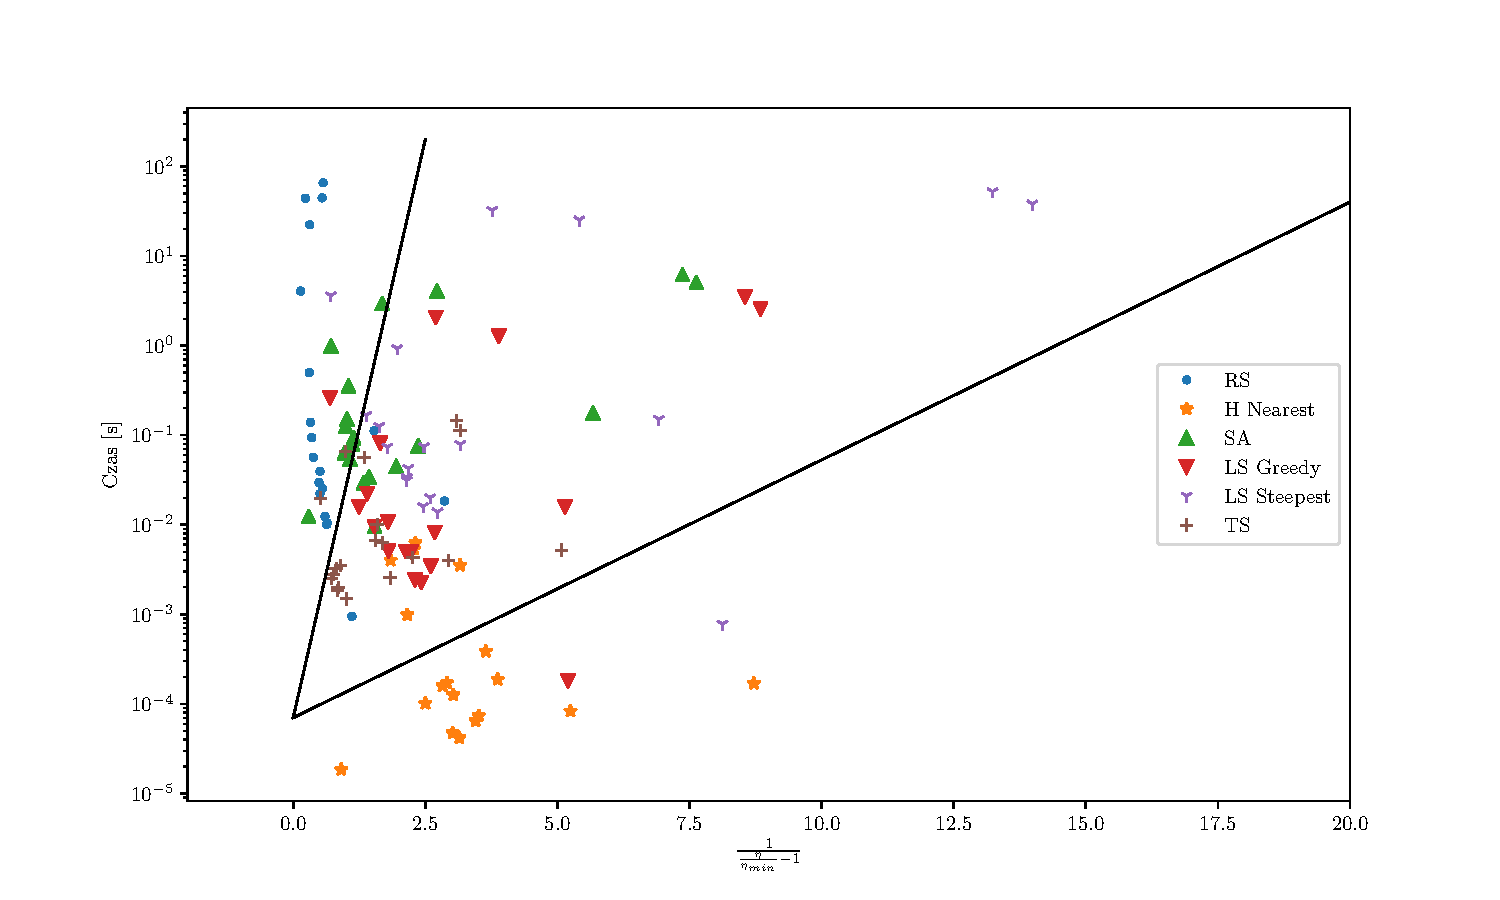
\includegraphics[width=1\textwidth]{quality.pdf}
\end{center}
\caption{Efektywność algorytmów}
\label{fig:plot_quality}
\end{figure}

Aby zbadać który algorytm jest najbardziej efektywny biorąc pod uwagę czas działania oraz jakoś wyniku wykreśliliśmy wykres punktowy który przedstawia te zależności. Aby znaleźć najefektywniejsze algorytmy należy spojrzeć na kąt pomiędzy początkiem układu współrzędnych, punktem odpowiadającym instancji, a osią X. Na wykres zostały naniesione linie dzielące podobne jakościowo algorytmy. Z rys. \ref{fig:plot_quality} można wyczytać że najlepsze wyniki w czasie uzyskał algorytm heurystyczny a najgorsze algorytm losowy.


\subsection{Średnia liczba kroków algorytmów}

\begin{figure} 
\begin{center}
    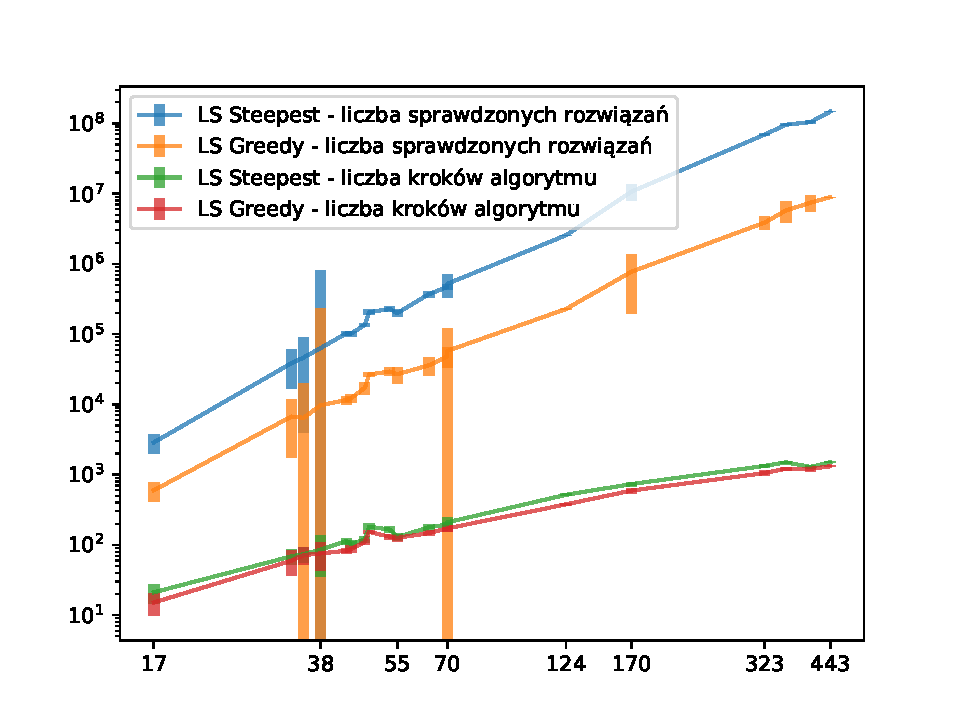
\includegraphics[width=1\textwidth]{steps2.pdf}
\end{center}
\caption{Średnia liczba kroków algorytmów}
\label{fig:plot_steps}
\end{figure}

Na rys. \ref{fig:plot_steps} przedstawiono ilość kroków i ilość obliczonych delt przez algorytmy Greedy i Steepest. Widać że instancje 33 i 38 miały bardzo różne ilości sprawdzonych rozwiązań przez algorytm greedy. Z danych wynika także że algorytm steepest sprawdzał więcej rozwiązań, zaś liczba kroków była podobna co może świadczyć o tym że nie opłaca się sprawdzać wszystkich sąsiadów aby trafić w podobne minimum lokalne co algorytm steepest, ponieważ wyniki tych algorytmów są podobne a czas działania lepszy w algorytmie greedy.




\begin{figure}[H]
    \begin{center}
        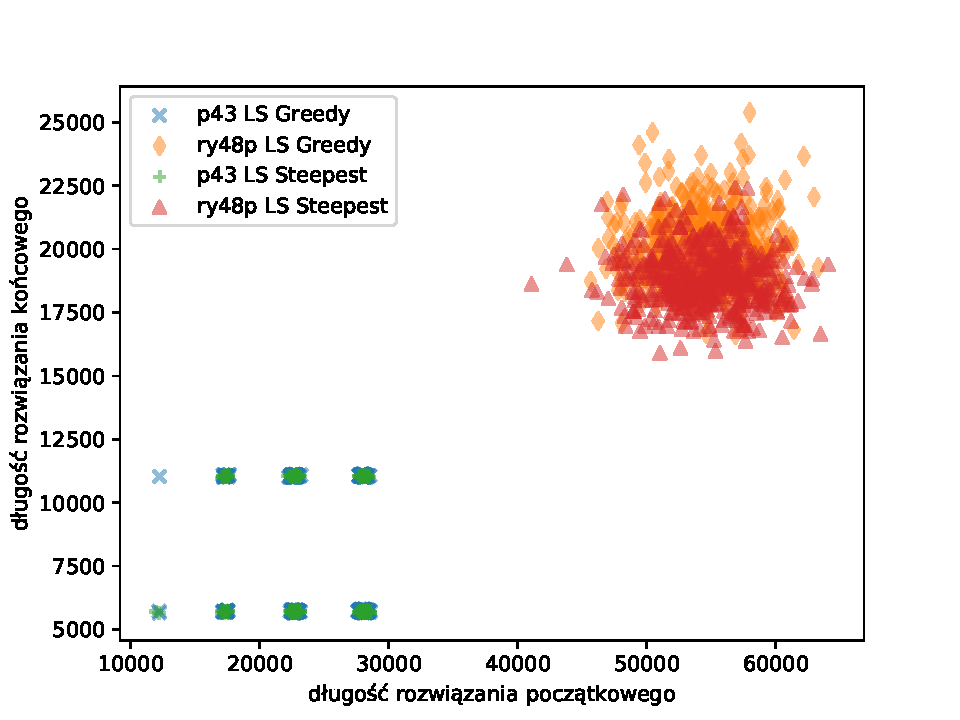
\includegraphics[width=1\textwidth]{first_last_finest.pdf}
    \end{center}
    \caption{Jakość rozwiązania początkowego, a jakość rozwiązania końcowego}
    \label{fig:first_finnest}
\end{figure}


\section{Jakość rozwiązania początkowego, a jakość rozwiązania końcowego}

Rys. \ref{fig:first_finnest} przedstawia zależność długości rozwiązania początkowego i długości rozwiązania końcowego dla instancji 43 i 48. Dla instancji 248 obydwa algorytmy dawały losowe rozwiązania z tym że algorytm steepest dawał nieco lepsze rezultaty. Dla instancji 48 oba algorytmy wpadały w podobne 4 minima lokalne i nie były wstanie polepszyć wyników. Dla tej instancji optimum lokalne miało długość 5620 co w części rozwiązań zostawało osiągane.

\section{Jakość rozwiązania w zależności od ilości uruchomień}

\begin{figure}[H]
    \begin{center}
        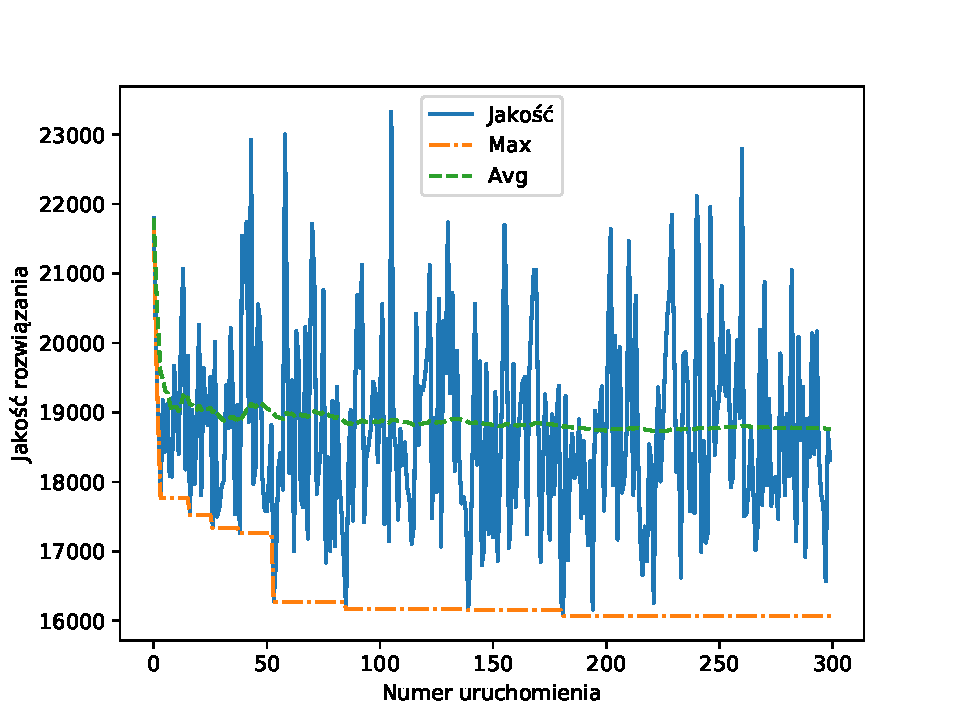
\includegraphics[width=1\textwidth]{multi_run_ry48p_atsp.pdf}
    \end{center}
    \caption{Jakość rozwiązania w zależności od ilości uruchomień. Instancja ry48p.}
    \label{fig:plot_multi_run_ry48p}
\end{figure}

\begin{figure}[H]
    \begin{center}
        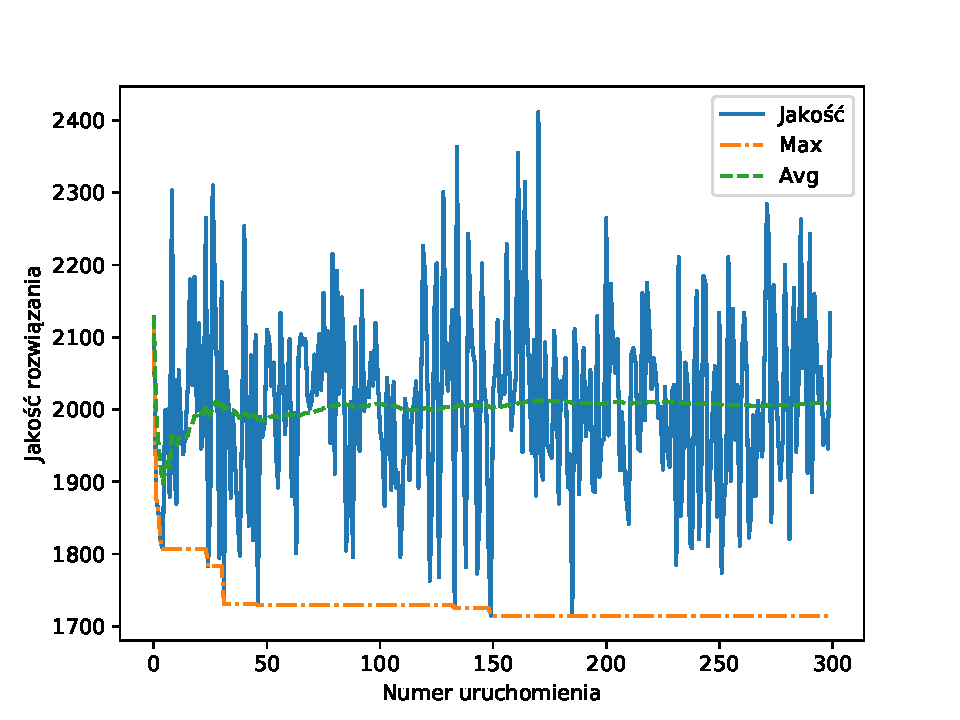
\includegraphics[width=1\textwidth]{multi_run_ftv35_atsp.pdf}
    \end{center}
    \caption{Jakość rozwiązania w zależności od ilości uruchomień. Instancja ftv35.}
    \label{fig:plot_multi_run_ftv35}
\end{figure}

Przedstawione na rys. \ref{fig:plot_multi_run_ry48p} i \ref{fig:plot_multi_run_ftv35}  wykresy przedstawiają jakość rozwiązania w zależności od liczby uruchomień, Z wykresów wynika że po ok 50 uruchomieniach obydwa algorytmy uzyskały drugie najlepsze wyniki spośród stu uruchomień. Na pewno można polepszyć wyniki ale widać że potrzebo ok dwukrotnie więcej uruchomień aby uzyskać 

\section{Podobieństwo rozwiązań}

Na rys. \ref{fig:quality_sim_ry48p} i \ref{fig:quality_sim_ftv48} pokazana jest zależność pomiędzy jakością 1000 rozwiązań a znalezionym optimum lokalnym. Można zauważyć że im lepsze rozwiązanie tym bardziej jest podobne do znalezionego optimum.

\begin{figure}[H]
    \begin{center}
        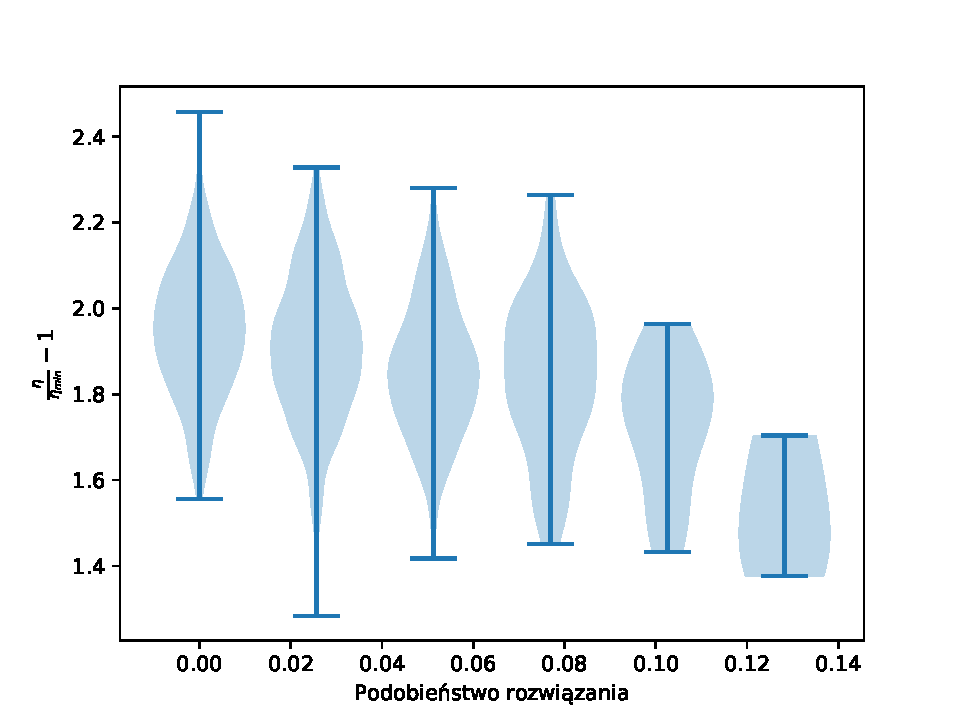
\includegraphics[width=1\textwidth]{quality_similarity_ftv38.pdf}
    \end{center}
    \caption{Jakość rozwiązania w zależności podobieństwa do znalezionego optimum. Instancja ftv38.}
    \label{fig:quality_sim_ftv38}
\end{figure}

\begin{figure}[H]
    \begin{center}
        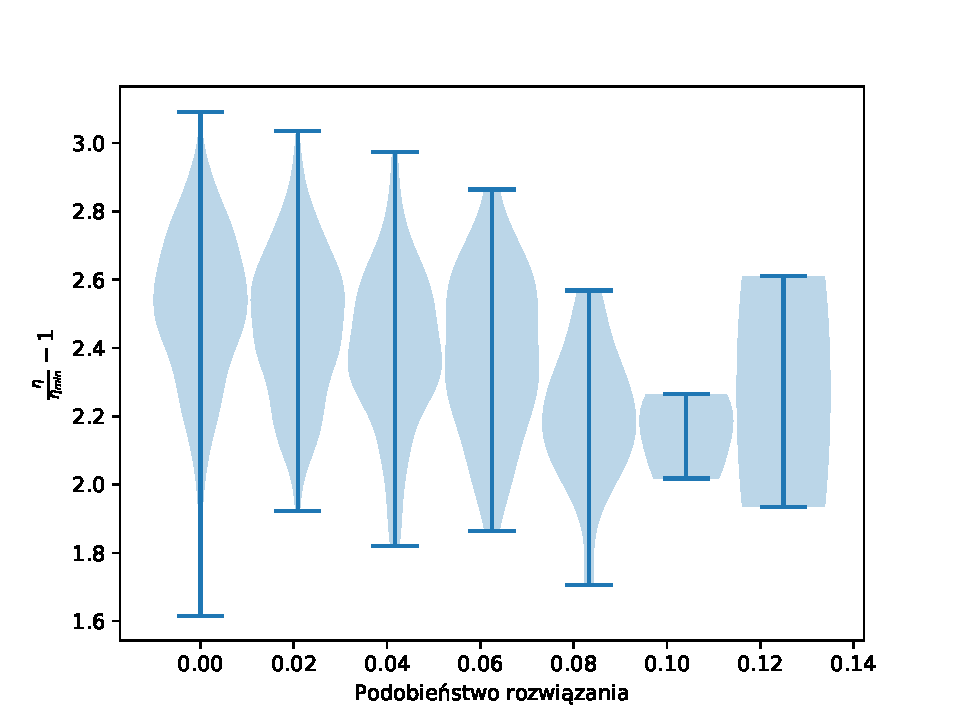
\includegraphics[width=1\textwidth]{quality_similarity_ry48p.pdf}
    \end{center}
    \caption{Jakość rozwiązania w zależności podobieństwa do znalezionego optimum. Instancja ry48p.}
    \label{fig:quality_sim_ry48p}
\end{figure}


Na rys. \ref{fig:quality_sim} przedstawiono podobieństwo 15 najlepszych spośród 1000 rozwiązań oraz ich podobieństwo do najlepszego znalezionego rozwiązania. Widać ze rozwiązania różnią się a najbardziej podobne są tylko w 12.5/%.


\begin{figure}[H]
    \begin{center}
        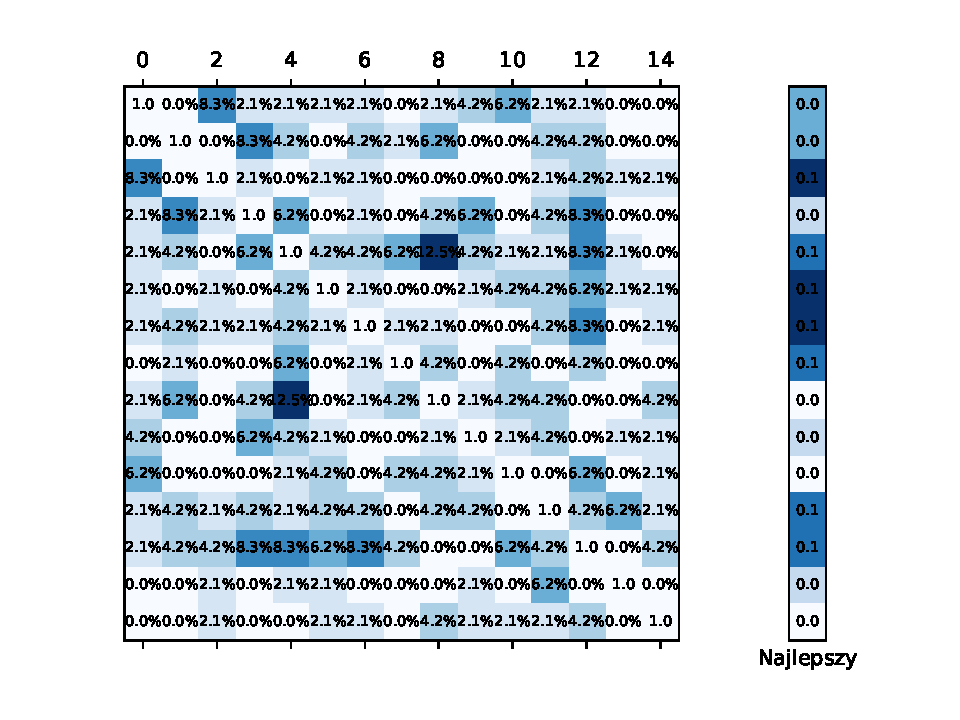
\includegraphics[width=1\textwidth]{quality_similarity_best15.pdf}
    \end{center}
    \caption{Podobieństwo 15 najlepszych rozwiązań oraz znalezionego optimum. Instancja ry48p.}
    \label{fig:quality_sim}
\end{figure}

\section{Wnioski}

Najlepiej sprawdził się algorytm heurystyczny który działał zarówno w najkrótszym czasie jak i dawał najlepsze wyniki. Algorytm losowy wypadł najgorzej. Speetest i Greedy dały podobne rezultaty z tym że steepest średnio dawał lepsze rozwiązania.

\section{Trudności i problemy}

Aby wykonać poprawnie wykresy i pokazać jak najwięcej informacji trzeba poświęcić dużo czasu na ich stworzenie. Początkowo pojawiły się także problemy z budowaniem części projektu napisanej w c++ gdyż wymaga on narzędzi w jednakowej wersji i konfiguracji.

\section{Propozycje udoskonaleń}

Można by dodać bibliotekę napisaną w języku cpp jako skompilowany moduł do języka Python co ułatwiłoby komunikację między językami.

\clearpage

\bibliography{report}
\bibliographystyle{plainurl}


\end{document}
